\documentclass{article}

\usepackage[landscape]{geometry}
\usepackage{tikz}
\usepackage[utf8]{inputenc}

%\usetikzlibrary{shapes, geometric, arrows}

\tikzstyle{process} = [rectangle, minimum width = 1.5cm, minimum height = 1cm, 
	text centered, ultra thick, draw = black]
\tikzstyle{arrow} = [ultra thick, ->]	

\begin{document}
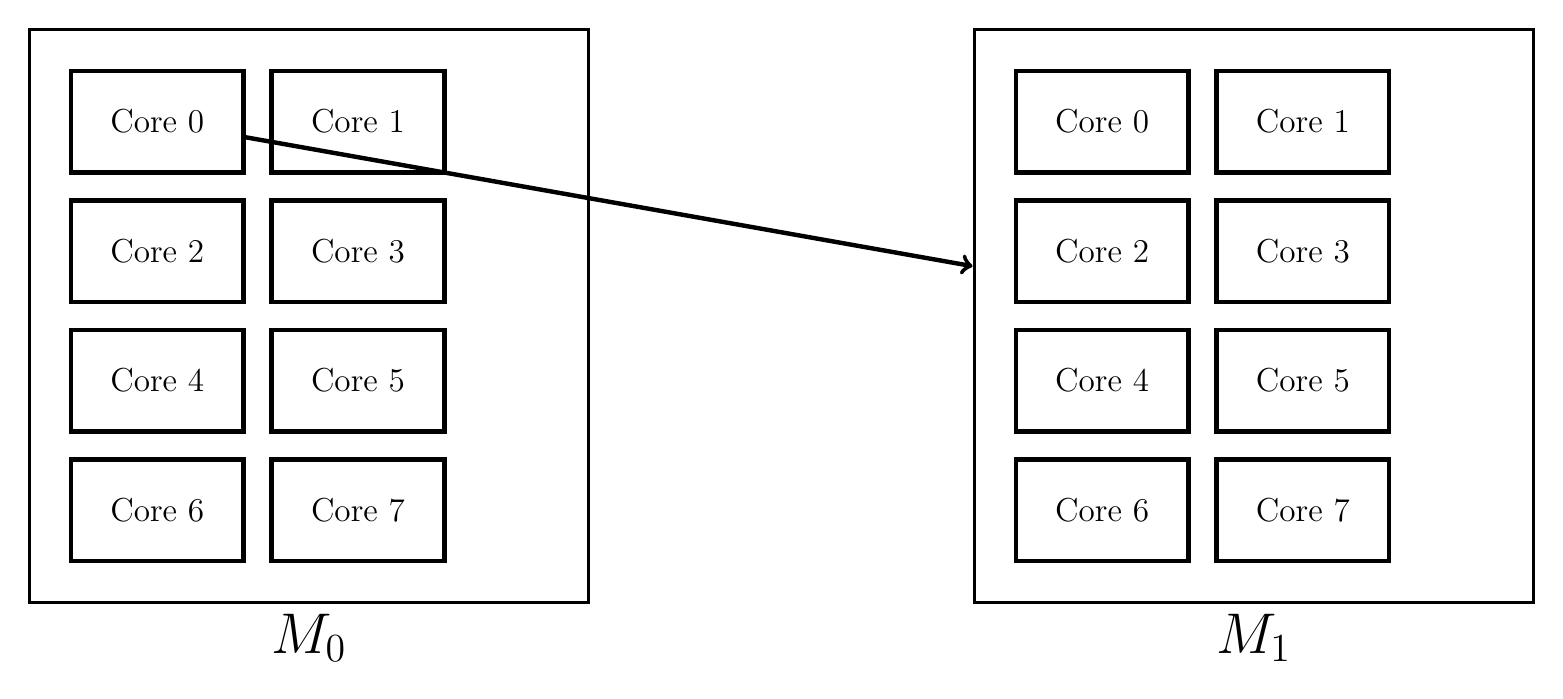
\begin{tikzpicture}[node distance = 12cm]

\node (M0) [matrix, draw = black, very thick, 
	inner sep = 5mm, row sep = 3mm, column sep = 3mm, 
	label = below:\huge $M_0$]
{
	\node (M00) [process] {\large Core 0}; & 
	\node (M01) [process] {\large Core 1}; &
	[1cm]\\

	\node (M02) [process] {\large Core 2}; & 
	\node (M03) [process] {\large Core 3}; &
	[1cm]\\

	\node (M04) [process] {\large Core 4}; & 
	\node (M05) [process] {\large Core 5}; &
	[1cm]\\

	\node (M06) [process] {\large Core 6}; & 
	\node (M07) [process] {\large Core 7}; &
	[1cm]\\
};


\node (M1) [matrix, draw = black, very thick, right of = M0, 
	inner sep = 5mm, row sep = 3mm, column sep = 3mm, 
	label = below:\huge $M_1$]
{
	\node (M10) [process] {\large Core 0}; & 
	\node (M11) [process] {\large Core 1}; &
	[1cm]\\

	\node (M12) [process] {\large Core 2}; & 
	\node (M13) [process] {\large Core 3}; &
	[1cm]\\

	\node (M14) [process] {\large Core 4}; & 
	\node (M15) [process] {\large Core 5}; &
	[1cm]\\

	\node (M16) [process] {\large Core 6}; & 
	\node (M17) [process] {\large Core 7}; &
	[1cm]\\
};

\draw [arrow] (M00) -- (M1);
\end{tikzpicture}
\end{document}
